\section{9 Oct 23 - Notes: Method of
Relaxation}\label{oct-23---notes-method-of-relaxation}

We've found a number of potential ways to solve Laplace's equation. All
of them have so far been analytical -- making use of special functions
and introducing basis functions to expand our solutions and develop
(potentially infinite) series solutions. As we saw with spherical
problems, this is a very powerful method to use, but it is not always
possible to find a solution in this way. In some cases you might be able
to find general solutions of the form (or in alternative coordinate
systems)):

\[\Phi(x,y,z)=X(x)Y(y)Z(z)\]

But nothing about Laplace's equation guarantees that such solutions are
possible. However, there are two major consequences of the solutions to
Laplace's Equation that give us a suggestion for a numerical approach.
These are because Laplace's equation is a linear, second order, partial
differential equation.

\begin{enumerate}
\def\labelenumi{\arabic{enumi}.}
\tightlist
\item
  The value of the potential at a point is the average of the potential
  at all points around it.
\item
  The solution that matches the boundary conditions is unique.
\end{enumerate}

So we can imagine taking a bubble or a sheet of rubber or plastic wrap
and stretching it over the region of interest. The shape and height of
the edges (barring the gravitational pull) set the shape of the
resulting bubble/sheet. Here we leave out gravity as it has a
directional pull, which Laplace's equation does not. The method we
propose below is called the
\href{https://en.wikipedia.org/wiki/Relaxation_(iterative_method)}{Method
of Relaxation}. It is a numerical method for solving PDEs where the
solution is determined iteratively using the two properties above.

\subsection{The Method of Relaxation}\label{the-method-of-relaxation}

The basic approach to the method of relaxation is laid out below:

\begin{enumerate}
\def\labelenumi{\arabic{enumi}.}
\tightlist
\item
  Divide the region into a grid of points. \emph{This is the
  discretization of the region. The smaller the grid, the more accurate
  the solution.} This is called ``a mesh'' in the literature.
\item
  Assign an initial value to each point in the grid. \emph{This is the
  initial guess for the solution.} This can be random or informed.
\item
  Set the value of each point on the boundary to the value expected by
  the boundary conditions. \emph{This is what makes this a boundary
  value problem.}
\item
  Step through each non-boundary point and set its value to the average
  values of the points around it. \emph{This is the relaxation step.}
\item
  Repeat step 4 until the values of the points stop changing. \emph{This
  is the convergence step.}
\end{enumerate}

There's a lot of nuance to these five steps, and we will get into this a
bit. Let's just write this up for the 1D problem.

\subsection{The 1 Dimensional Case}\label{the-1-dimensional-case}

Consider the 1D case of Laplace's equation:

\[\frac{d^2\Phi}{dx^2}=0\]

We can solve this problem quite easily, as we know the only non-zero
solution is a linear function.

\[\Phi(x)=ax+b\]

We can set the boundary conditions to be \(\Phi(0)=V_0\) and
\(\Phi(L)=0\) to find that \(b=V_0\) and \(a=-V_0/L\). So the solution
is:

\[\Phi(x)=-V_0\dfrac{x}{L}+V_0\]

It is a unique solution, and it is the average of the boundary
conditions (and also equally spaced points).

Let's solve it using the method of relaxation. Recall that:

\[f'(x)\approx \frac{f(x+a)+f(x-a)}{2}\]

so that,

\[f''(x)\approx \frac{f(x+a)-2f(x)+f(x-a)}{(a)^2}\]

So we can write Laplace's equation as:

\[\frac{\Phi(x+a)-2\Phi(x)+\Phi(x-a)}{(a)^2}=0\]

Or in terms of the grid spacing \(a\) starting at \(x_i\):

\[\Phi(x_i+a)-2\Phi(x_i)+\Phi(x_i-a)=0\]

So that we can solve for the value of \(V(x_i)\) at each point in the
grid.

\[\Phi(x_i)=\frac{1}{2}\left[\Phi(x_i+a)+\Phi(x_i-a)\right]\]

which is precisely the average of the value of the potential to the left
and right of the grid point. Let's write this in Python.

\begin{Shaded}
\begin{Highlighting}[]
\ImportTok{import}\NormalTok{ numpy }\ImportTok{as}\NormalTok{ np}
\ImportTok{import}\NormalTok{ matplotlib.pyplot }\ImportTok{as}\NormalTok{ plt}
\end{Highlighting}
\end{Shaded}

\begin{Shaded}
\begin{Highlighting}[]
\KeywordTok{def}\NormalTok{ relax(initial\_array, tolerance}\OperatorTok{=}\FloatTok{1e{-}6}\NormalTok{, n}\OperatorTok{=}\DecValTok{50}\NormalTok{):}
    \CommentTok{\textquotesingle{}\textquotesingle{}\textquotesingle{}Relaxation method for solving Laplace\textquotesingle{}s equation in 1D. }
\CommentTok{    Requires the initial array and the tolerance.\textquotesingle{}\textquotesingle{}\textquotesingle{}}
    
\NormalTok{    a }\OperatorTok{=}\NormalTok{ initial\_array.copy() }\CommentTok{\# to avoid overwriting the initial array}
\NormalTok{    convergence }\OperatorTok{=} \VariableTok{False} \CommentTok{\# to check if the solution has converged}
\NormalTok{    iterations }\OperatorTok{=} \DecValTok{0}  \CommentTok{\# to count the number of iterations}
\NormalTok{    arrays }\OperatorTok{=}\NormalTok{ [a.copy()]  }\CommentTok{\# to store the array at each iteration}
    \ControlFlowTok{while} \KeywordTok{not}\NormalTok{ convergence:}
        
        \CommentTok{\# Compute the average of the two neighboring points}
        \CommentTok{\# as long as they are not boundaries}
        \CommentTok{\# and do so until you reach the desired tolerance}
\NormalTok{        iterations }\OperatorTok{+=} \DecValTok{1}
\NormalTok{        new\_a }\OperatorTok{=}\NormalTok{ a.copy()}
        
        \CommentTok{\# Computing the average of the two neighboring points}
        \ControlFlowTok{for}\NormalTok{ i }\KeywordTok{in} \BuiltInTok{range}\NormalTok{(}\DecValTok{1}\NormalTok{, }\BuiltInTok{len}\NormalTok{(a) }\OperatorTok{{-}} \DecValTok{1}\NormalTok{):  }\CommentTok{\# Excluding boundaries}
\NormalTok{            new\_a[i] }\OperatorTok{=} \FloatTok{0.5} \OperatorTok{*}\NormalTok{ (a[i }\OperatorTok{{-}} \DecValTok{1}\NormalTok{] }\OperatorTok{+}\NormalTok{ a[i }\OperatorTok{+} \DecValTok{1}\NormalTok{])}
        
        \CommentTok{\# checking if the solution has converged (i.e., achieved the desired tolerance)}
        \CommentTok{\# this is point by point convergence (See why?)}
\NormalTok{        convergence }\OperatorTok{=}\NormalTok{ np.}\BuiltInTok{all}\NormalTok{(np.}\BuiltInTok{abs}\NormalTok{(new\_a }\OperatorTok{{-}}\NormalTok{ a) }\OperatorTok{\textless{}}\NormalTok{ tolerance)}
        
\NormalTok{        a }\OperatorTok{=}\NormalTok{ new\_a.copy()}
        
        \CommentTok{\# store every nth iteration (default is 50)}
        \ControlFlowTok{if}\NormalTok{ iterations }\OperatorTok{\%}\NormalTok{ n }\OperatorTok{==} \DecValTok{0}\NormalTok{:}
\NormalTok{            arrays.append(a.copy())}
    
    \ControlFlowTok{return}\NormalTok{ arrays, iterations}
\end{Highlighting}
\end{Shaded}

\begin{Shaded}
\begin{Highlighting}[]
\KeywordTok{def}\NormalTok{ plot\_relaxation(arrays, total\_iterations):}
    \BuiltInTok{print}\NormalTok{(}\SpecialStringTok{f\textquotesingle{}The solution converged after }\SpecialCharTok{\{}\NormalTok{total\_iterations}\SpecialCharTok{\}}\SpecialStringTok{ iterations.\textquotesingle{}}\NormalTok{)}

    \CommentTok{\# Set up the figure and axis}
\NormalTok{    fig, ax }\OperatorTok{=}\NormalTok{ plt.subplots(figsize}\OperatorTok{=}\NormalTok{(}\DecValTok{8}\NormalTok{, }\DecValTok{6}\NormalTok{))}
\NormalTok{    colors }\OperatorTok{=}\NormalTok{ plt.cm.viridis(np.linspace(}\DecValTok{0}\NormalTok{, }\DecValTok{1}\NormalTok{, }\BuiltInTok{len}\NormalTok{(arrays)))  }\CommentTok{\# Create a colormap for the iterations}

    \ControlFlowTok{for}\NormalTok{ i, array }\KeywordTok{in} \BuiltInTok{enumerate}\NormalTok{(arrays):}
\NormalTok{        ax.plot(array, color}\OperatorTok{=}\NormalTok{colors[i], label}\OperatorTok{=}\SpecialStringTok{f\textquotesingle{}Iteration: }\SpecialCharTok{\{}\NormalTok{i}\SpecialCharTok{\}}\SpecialStringTok{\textquotesingle{}}\NormalTok{)}
    
\NormalTok{    ax.set\_title(}\StringTok{\textquotesingle{}Relaxation Method: Overlaid Iterations\textquotesingle{}}\NormalTok{)}
\NormalTok{    ax.set\_xlabel(}\StringTok{\textquotesingle{}Position (x)\textquotesingle{}}\NormalTok{)}
\NormalTok{    ax.set\_ylabel(}\StringTok{\textquotesingle{}Electric Potential (V)\textquotesingle{}}\NormalTok{)}
    
    \ControlFlowTok{return}\NormalTok{ fig, ax}
\end{Highlighting}
\end{Shaded}

\begin{Shaded}
\begin{Highlighting}[]
\NormalTok{N }\OperatorTok{=} \DecValTok{100} \CommentTok{\# number of grid points}
\NormalTok{arr }\OperatorTok{=}\NormalTok{ np.zeros(N) }\CommentTok{\# initial array}
\NormalTok{tol }\OperatorTok{=} \FloatTok{1e{-}6} \CommentTok{\# tolerance}
\NormalTok{n }\OperatorTok{=} \DecValTok{50} \CommentTok{\# store every nth iteration}

\CommentTok{\# Boundary conditions}
\NormalTok{arr[}\DecValTok{0}\NormalTok{] }\OperatorTok{=} \DecValTok{100} \CommentTok{\# left boundary (100 V)}
\NormalTok{arr[}\OperatorTok{{-}}\DecValTok{1}\NormalTok{] }\OperatorTok{=} \DecValTok{0} \CommentTok{\# right boundary (0 V)}

\NormalTok{arrays, total\_iterations }\OperatorTok{=}\NormalTok{ relax(arr, tol, n)}
\NormalTok{plot\_relaxation(arrays, total\_iterations)}\OperatorTok{;}
\end{Highlighting}
\end{Shaded}

\begin{verbatim}
The solution converged after 21980 iterations.
\end{verbatim}

\begin{figure}
\centering
\pandocbounded{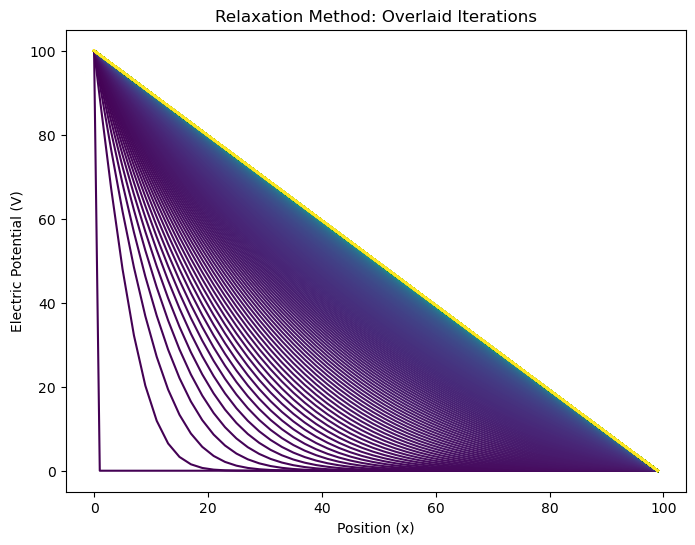
\includegraphics[keepaspectratio,alt={png}]{../images/notes-relaxation_notes-relaxation_tmp_5_1.png}}
\caption{png}
\end{figure}

\subsubsection{Experiments}\label{experiments}

We can change the number of grid points, the number of iterations, and
the initial guess to see how the solution changes; in particular, how
quickly the solution converges.

\paragraph{Random Initial Guess}\label{random-initial-guess}

\begin{Shaded}
\begin{Highlighting}[]
\NormalTok{N }\OperatorTok{=} \DecValTok{100} \CommentTok{\# number of grid points}
\NormalTok{arr }\OperatorTok{=}\NormalTok{ np.random.rand(N) }\CommentTok{\# initial array}
\NormalTok{tol }\OperatorTok{=} \FloatTok{1e{-}6} \CommentTok{\# tolerance}
\NormalTok{n }\OperatorTok{=} \DecValTok{50} \CommentTok{\# store every nth iteration}

\CommentTok{\# Boundary conditions}
\NormalTok{arr[}\DecValTok{0}\NormalTok{] }\OperatorTok{=} \DecValTok{100} \CommentTok{\# left boundary (100 V)}
\NormalTok{arr[}\OperatorTok{{-}}\DecValTok{1}\NormalTok{] }\OperatorTok{=} \DecValTok{0} \CommentTok{\# right boundary (0 V)}

\NormalTok{arrays, total\_iterations }\OperatorTok{=}\NormalTok{ relax(arr, tol, n)}
\NormalTok{plot\_relaxation(arrays, total\_iterations)}\OperatorTok{;}
\end{Highlighting}
\end{Shaded}

\begin{verbatim}
The solution converged after 25315 iterations.
\end{verbatim}

\begin{figure}
\centering
\pandocbounded{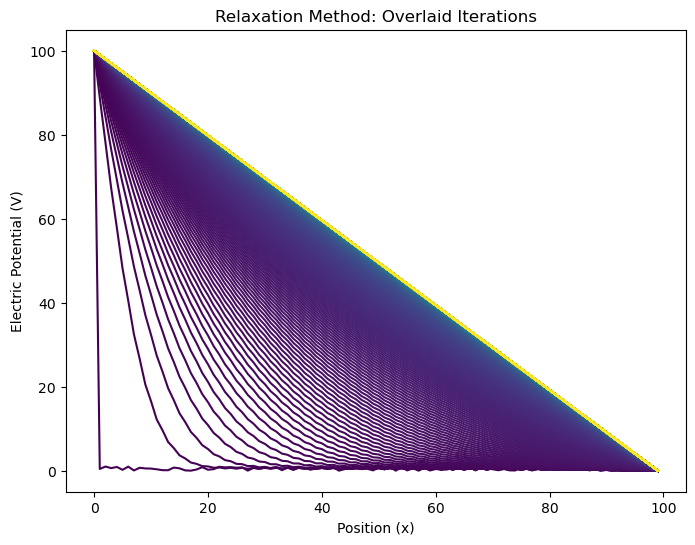
\includegraphics[keepaspectratio,alt={png}]{../images/notes-relaxation_notes-relaxation_tmp_7_1.png}}
\caption{png}
\end{figure}

\paragraph{Sinusoidal Initial Guess}\label{sinusoidal-initial-guess}

\begin{Shaded}
\begin{Highlighting}[]
\NormalTok{N }\OperatorTok{=} \DecValTok{100} \CommentTok{\# number of grid points}
\NormalTok{x }\OperatorTok{=}\NormalTok{ np.linspace(}\DecValTok{0}\NormalTok{, }\DecValTok{2}\OperatorTok{*}\NormalTok{np.pi, N)}
\NormalTok{arr }\OperatorTok{=} \DecValTok{50}\OperatorTok{*}\NormalTok{np.sin(x) }\CommentTok{\# initial array}
\NormalTok{tol }\OperatorTok{=} \FloatTok{1e{-}6} \CommentTok{\# tolerance}
\NormalTok{n }\OperatorTok{=} \DecValTok{50} \CommentTok{\# store every nth iteration}

\CommentTok{\# Boundary conditions}
\NormalTok{arr[}\DecValTok{0}\NormalTok{] }\OperatorTok{=} \DecValTok{100} \CommentTok{\# left boundary (100 V)}
\NormalTok{arr[}\OperatorTok{{-}}\DecValTok{1}\NormalTok{] }\OperatorTok{=} \DecValTok{0} \CommentTok{\# right boundary (0 V)}

\NormalTok{arrays, total\_iterations }\OperatorTok{=}\NormalTok{ relax(arr, tol, n)}
\NormalTok{plot\_relaxation(arrays, total\_iterations)}\OperatorTok{;}
\end{Highlighting}
\end{Shaded}

\begin{verbatim}
The solution converged after 21980 iterations.
\end{verbatim}

\begin{figure}
\centering
\pandocbounded{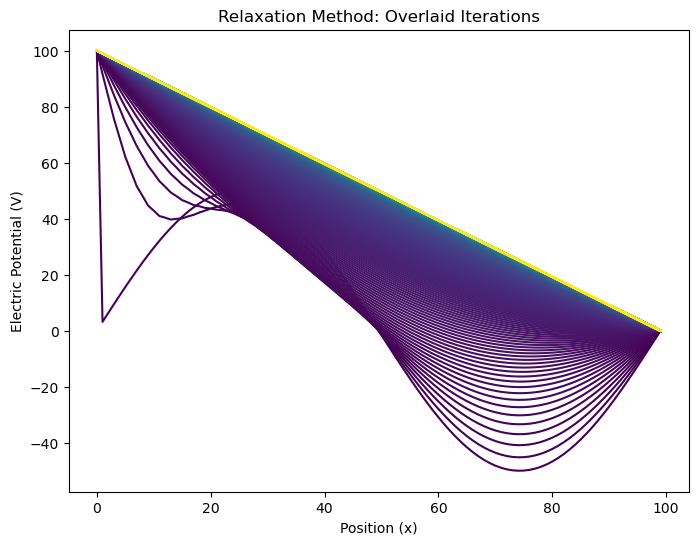
\includegraphics[keepaspectratio,alt={png}]{../images/notes-relaxation_notes-relaxation_tmp_9_1.png}}
\caption{png}
\end{figure}

\paragraph{Linear Initial Guess}\label{linear-initial-guess}

\begin{Shaded}
\begin{Highlighting}[]
\NormalTok{N }\OperatorTok{=} \DecValTok{100} \CommentTok{\# number of grid points}
\NormalTok{x }\OperatorTok{=}\NormalTok{ np.linspace(}\DecValTok{0}\NormalTok{, N, N)}
\NormalTok{arr }\OperatorTok{=} \OperatorTok{{-}}\NormalTok{x}\OperatorTok{+}\DecValTok{100} \CommentTok{\# initial array}
\NormalTok{tol }\OperatorTok{=} \FloatTok{1e{-}6} \CommentTok{\# tolerance}
\NormalTok{n }\OperatorTok{=} \DecValTok{50} \CommentTok{\# store every nth iteration}

\CommentTok{\# Boundary conditions}
\NormalTok{arr[}\DecValTok{0}\NormalTok{] }\OperatorTok{=} \DecValTok{100} \CommentTok{\# left boundary (100 V)}
\NormalTok{arr[}\OperatorTok{{-}}\DecValTok{1}\NormalTok{] }\OperatorTok{=} \DecValTok{0} \CommentTok{\# right boundary (0 V)}

\NormalTok{arrays, total\_iterations }\OperatorTok{=}\NormalTok{ relax(arr, tol, n)}
\NormalTok{plot\_relaxation(arrays, total\_iterations)}\OperatorTok{;}
\end{Highlighting}
\end{Shaded}

\begin{verbatim}
The solution converged after 1 iterations.
\end{verbatim}

\begin{figure}
\centering
\pandocbounded{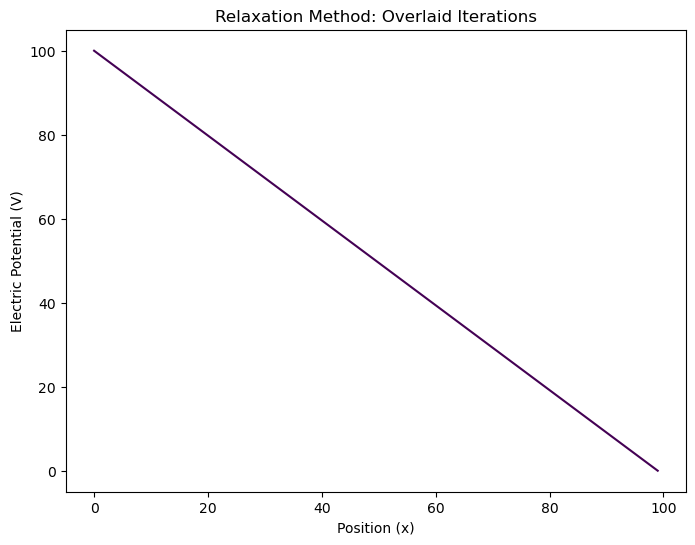
\includegraphics[keepaspectratio,alt={png}]{../images/notes-relaxation_notes-relaxation_tmp_11_1.png}}
\caption{png}
\end{figure}

\paragraph{Linear Initial Guess with a touch of white
noise}\label{linear-initial-guess-with-a-touch-of-white-noise}

\begin{Shaded}
\begin{Highlighting}[]
\NormalTok{N }\OperatorTok{=} \DecValTok{100} \CommentTok{\# number of grid points}
\NormalTok{x }\OperatorTok{=}\NormalTok{ np.linspace(}\DecValTok{0}\NormalTok{, N, N)}
\NormalTok{gamma }\OperatorTok{=} \DecValTok{2} \CommentTok{\# strength of noise}
\NormalTok{arr }\OperatorTok{=} \OperatorTok{{-}}\NormalTok{x}\OperatorTok{+}\DecValTok{100}\OperatorTok{+}\NormalTok{gamma}\OperatorTok{*}\NormalTok{np.random.rand() }\CommentTok{\# initial array}
\NormalTok{tol }\OperatorTok{=} \FloatTok{1e{-}6} \CommentTok{\# tolerance}
\NormalTok{n }\OperatorTok{=} \DecValTok{50} \CommentTok{\# store every nth iteration}

\CommentTok{\# Boundary conditions}
\NormalTok{arr[}\DecValTok{0}\NormalTok{] }\OperatorTok{=} \DecValTok{100} \CommentTok{\# left boundary (100 V)}
\NormalTok{arr[}\OperatorTok{{-}}\DecValTok{1}\NormalTok{] }\OperatorTok{=} \DecValTok{0} \CommentTok{\# right boundary (0 V)}

\NormalTok{arrays, total\_iterations }\OperatorTok{=}\NormalTok{ relax(arr, tol, n)}
\NormalTok{plot\_relaxation(arrays, total\_iterations)}\OperatorTok{;}
\end{Highlighting}
\end{Shaded}

\begin{verbatim}
The solution converged after 6285 iterations.
\end{verbatim}

\begin{figure}
\centering
\pandocbounded{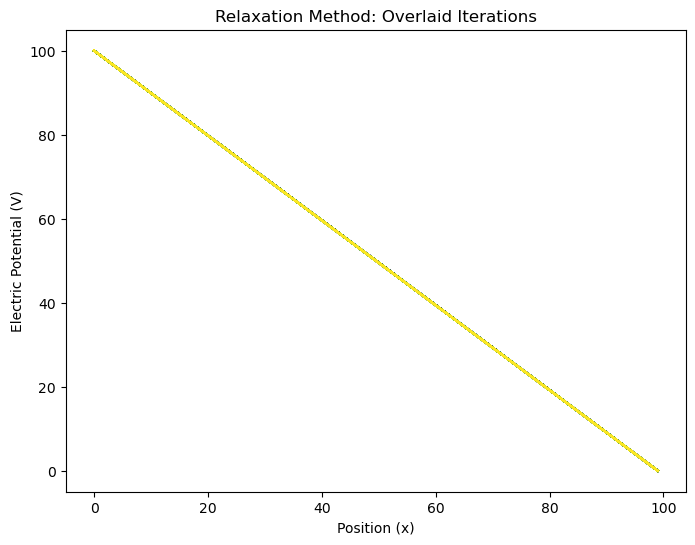
\includegraphics[keepaspectratio,alt={png}]{../images/notes-relaxation_notes-relaxation_tmp_13_1.png}}
\caption{png}
\end{figure}

\paragraph{Random Initial Guess with lower
tolerance}\label{random-initial-guess-with-lower-tolerance}

\begin{Shaded}
\begin{Highlighting}[]
\NormalTok{N }\OperatorTok{=} \DecValTok{100} \CommentTok{\# number of grid points}
\NormalTok{arr }\OperatorTok{=}\NormalTok{ np.random.rand(N) }\CommentTok{\# initial array}
\NormalTok{tol }\OperatorTok{=} \FloatTok{1e{-}3} \CommentTok{\# tolerance}
\NormalTok{n }\OperatorTok{=} \DecValTok{50} \CommentTok{\# store every nth iteration}

\CommentTok{\# Boundary conditions}
\NormalTok{arr[}\DecValTok{0}\NormalTok{] }\OperatorTok{=} \DecValTok{100} \CommentTok{\# left boundary (100 V)}
\NormalTok{arr[}\OperatorTok{{-}}\DecValTok{1}\NormalTok{] }\OperatorTok{=} \DecValTok{0} \CommentTok{\# right boundary (0 V)}

\NormalTok{arrays, total\_iterations }\OperatorTok{=}\NormalTok{ relax(arr, tol, n)}
\NormalTok{plot\_relaxation(arrays, total\_iterations)}\OperatorTok{;}
\end{Highlighting}
\end{Shaded}

\begin{verbatim}
The solution converged after 9413 iterations.
\end{verbatim}

\begin{figure}
\centering
\pandocbounded{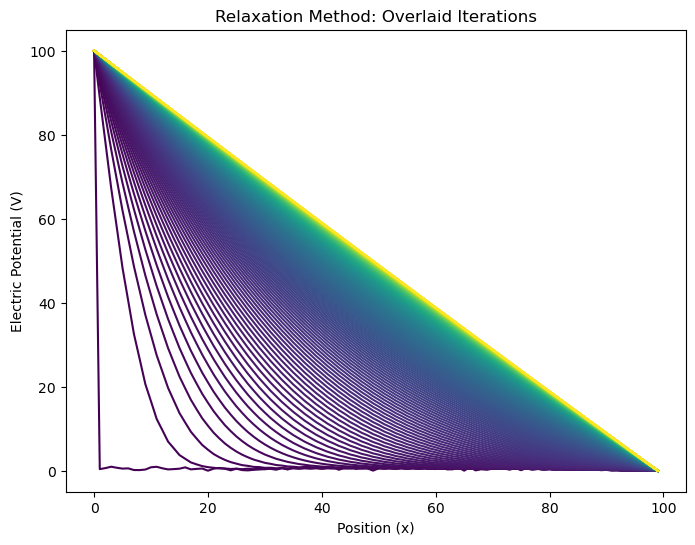
\includegraphics[keepaspectratio,alt={png}]{../images/notes-relaxation_notes-relaxation_tmp_15_1.png}}
\caption{png}
\end{figure}

\subsection{Relaxation Method in 2D}\label{relaxation-method-in-2d}

The two-dimensional case is a bit more complicated but it follows the
same basic idea. You will write the code to solve a problem like this,
but the underlying mathematics follows from our discretization of the
Laplacian. Maxwell's equations give us Laplace's equation for potential
\(\Phi\) with no source charges:

\[\nabla^2 \Phi = 0 \]

in two-dimensional Cartesian coordinates, this reads:

\[
\frac{\partial^2 \Phi}{\partial x^2} + \frac{\partial^2 \Phi}{\partial y^2} = 0.
\]

We're choosing the 2D version simply because it is easier to visualize.
Because this is a PDE, we will need to specify \textbf{boundary
conditions} for \(\Phi\) along the edges of the box as opposed to
initial conditions like we've seen for ODEs. Let's choose \(\Phi = V_0\)
along the top of the box and \(\Phi = 0\) on the other sides.

Numerically we can approximate the 2nd partial x derivative of \(\Phi\)
as:

\[
\frac{\partial^2 \Phi}{\partial x^2} \approx \frac{\Phi(x+h,y) + \Phi(x-h,y) - 2\Phi(x,y)}{h^2}
\]

for some small positive real number \(h\).

We can write this for the y direction as well:

\[
\frac{\partial^2 \Phi}{\partial y^2} \approx \frac{\Phi(x,y+h) + \Phi(x,y-h) - 2\Phi(x,y)}{h^2}
\]

Adding these gives us Laplace's equation:

\[
\frac{\partial^2 \Phi}{\partial x^2} + \frac{\partial^2 \Phi}{\partial y^2}  = \frac{\Phi(x+h,y) + \Phi(x-h,y) - 2\Phi(x,y) + \Phi(x,y+h) + \Phi(x,y-h) - 2\Phi(x,y)}{h^2} = 0 
\]

or more simply:

\[
\Phi(x+h,y) + \Phi(x-h,y) + \Phi(x,y+h) + \Phi(x,y-h) - 4\Phi(x,y)= 0 
\]

We want to know \(\Phi(x,y)\) and this equation thankfully has a
\(\Phi(x,y)\) term so we can solve for it:

\[
\Phi(x,y) = \frac{1}{4}\left[\Phi(x+h,y) + \Phi(x-h,y) + \Phi(x,y+h) + \Phi(x,y-h) \right]
\]

This is saying that we can approximate \(\Phi(x,y)\) by the average of
the grid points that surround it, which should feel intuitive. Here
comes the clever bit for how we turn this into a solver - We first the
boundary points of our grid to our boundary conditions and set all the
interior points to zero. Then we use this equation to update each
interior point by its neighbors, that is:

\[
\Phi_{k+1}(x,y) = \frac{1}{4}\left[\Phi_{k}(x+h,y) + \Phi_{k}(x-h,y) + \Phi_{k}(x,y+h) + \Phi_{k}(x,y-h) \right]
\]

Then we iterate this process, for many values of \(i\) until our system
converges (If it converges! This method isn't guarenteed to converge.).
To check for convergence, we can calculate the change
\(\delta = |\Phi_{k+1}(x,y) - \Phi(x,y)|\) and terminate the algorithm
when \(\delta\) is sufficiently small.

It might seem fairly obvious that the 3D version of this is just an
extension of the 2D version, and it is. The 3D version is:

\[\Phi_{k+1}(x,y,z) = \frac{1}{6}\left[\Phi_{k}(x+h,y,z) + \Phi_{k}(x-h,y,z) + \Phi_{k}(x,y+h,z) + \Phi_{k}(x,y-h,z) + \Phi_{k}(x,y,z+h) + \Phi_{k}(x,y,z-h) \right]\]

\subsection{Additional Resources}\label{additional-resources}

\subsubsection{Handwritten Notes}\label{handwritten-notes}

\begin{itemize}
\tightlist
\item
  \href{../../assets/notes/Notes_Laplaces_Equation.pdf}{Laplace's
  Equation}
\item
  \href{../../assets/notes/Notes-Method_of_Relaxation.pdf}{Method of
  Relaxation}
\end{itemize}

\subsubsection{Videos}\label{videos}

These videos from 3Blue1Brown about Partial Differential Equations are
really great. But not necessary to grasp what we are doing.

\href{https://inv.tux.pizza/watch?v=ly4S0oi3Yz8}{\pandocbounded{\includegraphics[keepaspectratio,alt={What is a PDE}]{https://markdown-videos-api.jorgenkh.no/youtube/ly4S0oi3Yz8?width=720&height=405}}}

\begin{itemize}
\tightlist
\item
  Non-Commercial Link: \url{https://inv.tux.pizza/watch?v=ly4S0oi3Yz8}
\item
  Commercial Link: \url{https://youtube.com/watch?v=ly4S0oi3Yz8}
\end{itemize}

\href{https://inv.tux.pizza/watch?v=ToIXSwZ1pJU}{\pandocbounded{\includegraphics[keepaspectratio,alt={Solving the Heat Equation}]{https://markdown-videos-api.jorgenkh.no/youtube/ToIXSwZ1pJU?width=720&height=405}}}

\begin{itemize}
\tightlist
\item
  Non-Commercial Link: \url{https://inv.tux.pizza/watch?v=ToIXSwZ1pJU}
\item
  Commercial Link: \url{https://youtube.com/watch?v=ToIXSwZ1pJU}
\end{itemize}
